% mainfile: ../../Refinement.tex
\subsubsection{Parallel composition}
\label{sec_comp_par}
To show the compositionality of the parallel operator for processes without restriction and recursion, we take advantage of the at most countable infinity number of traces within a trace set. Thus, we can uniquely index every trace of a process $P$ and a process $Q$ to reach their indexed trace sets. Because of those indices we can remember which traces of $P$ and $Q$ are used to gain the behavior of the composition in an inductive calculation. This intuition is visualized in \refFig{fig_exp_comp_para}.

% mainfile: ../Refinement.tex
\begin{figure}[h]
\centering
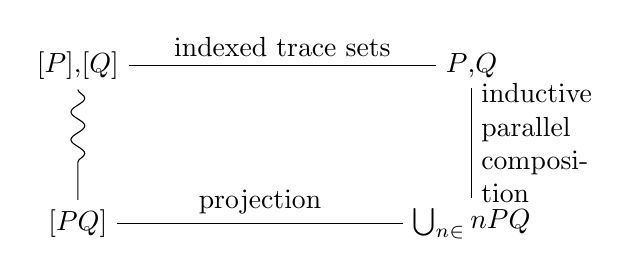
\begin{tikzpicture}
	\node   			(A)	{$\traces[P]$,$\traces[Q]$};
	\node[right of=A, xshift=40mm]	(B)	{$\trI{P}$,$\trI{Q}$};
	\node[below of=B, yshift=-10mm]		(C)	{$\bigcup_{n\in\N}\tracesI{n}{P}{Q}$};
	\node[below of=A, yshift=-10mm]		(D)	{$\traces[\procpar{P}{Q}]$};
	\path	(A)    edge node[anchor=south]  {indexed trace sets}            (B)
		(B)    edge node[anchor=west, text width=15mm]   {inductive parallel composition}    (C)
		(C)    edge node[anchor=south]  {projection}		(D);
	\path	(A)    edge[draw,decorate,decoration={snake, post=lineto, post length=4mm}] 
			    node[anchor=east]   {} (D);
\end{tikzpicture}
\caption{Visualization of the compositionality of the parallel operator (Part I).}
\label{fig_exp_comp_para}
\end{figure}


The behavior of a parallel composition of two processes is their interleaving behavior and the behavior originated from the possible communications between those two processes. For the calculation of the behavior of a parallel composition it is very helpful that we only investigate processes without any restriction operators. Thus, no bound action can exist in any trace. Hence, we neither have to attend to the side condition of the \eparl{} respectively \eparr{} rule for the interleaving behavior nor mind the \eclosel{} respectively \ecloser{} rule of \refFig{fig_ts_early} for the communication case.

Note that for the construction of the additional behavior originated of the communications, we do not have the same problem as described for the case of an input process. This is because in this case, we do have the information to which process the actions belong by calculating the communication behavior.

Following the intuition, we first inductively define the \findex{inductive parallel composition} of a parallel composition by using the indexed trace sets of the components. That is, we memorize from which trace of the one and the other process in the parallel composition the trace of the parallel composed process is constructed and how many of the actions from the traces are used for this construction.

\begin{definition}[Inductive parallel composition]
\label{def_idx_trace_sets}
Let $P,Q\in\procsresf\cap\procsrecf$. Then the function family $\traces_n:\procs_\alpha \rightarrow \pom{(\N^2\times\N^2)\times\tr}$ is defined with
\begin{align*}
	 \tracesI{0}{P}{Q} \define& \set[i_P,i_Q\in\N]{\left(\left(\left(i_P,0\right),\left(i_Q,0\right)\right),\eseq\right)} \\
	 \tracesI{n+1}{P}{Q} \define& \bigl\{\left(\left(\left(i_P,j_P\right),\left(i_Q,j_Q\right)\right),s'\right)\in (\N^2\times\N^2)\times\tr \; \mid \; \\
		& \quad\quad\exists\left(\left(\left(i_P,j_P'\right),\left(i_Q,j_Q'\right)\right),t'\right)\in\tracesI{n}{P}{Q}, \\
		& \quad\quad\quad \left(i_P,s\right)\in\trI{P}, \left(i_Q,t\right)\in\trI{Q}: \\
		& \quad\quad \text{PL}\define\left(j_P=j_P'+1\wedge j_Q=j_Q'\wedge s'=\seqconc{t'}{\seq{s_{j_P}}}\right) \\
		& \quad\wedge \text{PR}\define\left(j_P=j_P'\wedge j_Q=j_Q'+1\wedge s'=\seqconc{t'}{\seq{t_{j_Q}}}\right)  \\
		& \quad\wedge \text{COM}\define\left(j_P=j_P'+1\wedge j_Q=j_Q'+1\wedge s_{j_P}=\conj{t_{j_Q}}\wedge s'=t'\right)\\
		& \quad\wedge \left(\text{PR} \vee \text{PL} \vee \text{COM}\right) \bigr\}
\end{align*}
by induction over $n\in\N$.
\end{definition}

Thus, for a trace $t\in\tr$ of a parallel composition $\procpar{P}{Q}\in\procsresf\cap\procsrecf$, we save the index $i_P$ as well as the index $i_Q$ to memorize from which trace of $P$ respectively $Q$ the trace $t$ is constructed. Additionally, we save with $j_P$ and $j_Q$ the index within the trace of $P$ respectively $Q$, till this index the trace is used for the construction.

Note that the index of the sets does not map the length of the containing traces, since with the conjunctive clause COM every $\tau$ step raises the index, but does not extend the trace. We just can say that for a trace $t\in\tracesI{n}{P}{Q}$ the inequality $\len{t}\leq{}n$ holds. Moreover, the index $n$ counts the inference steps of the operational semantics which had been done to reach the actual tuple of indices and trace.

We now connect this definition to the big-step semantics to have a tool for proving the compositionality of the parallel composition of restriction and recursion free processes.

\begin{lemma}[Inductive parallel composition with big-step semantics]
\label{lem_idx_trace_sets}
$\quad$\newline{}Let $P,Q\in\procsresf\cap\procsrecf$. Then for all $n\in\N\setminus\set{0}$:\newline
\newline
if a tuple $\left(\left(\left(i_P,j_P\right),\left(i_Q,j_Q\right)\right),s'\right)\in\tracesI{n}{P}{Q}$ exists, then there are tuples
\begin{align*}
  \left(\left(\left(i_P,j_P'\right),\left(i_Q,j_Q'\right)\right),t'\right)&\in\tracesI{n-1}{P}{Q}, \\
  \left(i_P,s\right)&\in\trI{P},\\
  \left(i_Q,t\right)&\in\trI{Q}
\end{align*}
such that
\begin{align*}
	&\bigl(j_P=j_P'+1\wedge j_Q=j_Q'\wedge s'=\seqconc{t'}{\seq{s_{j_P}}}\wedge\exists P_1,P_2,Q_1\in\procs: \\
 &\quad\ec{P}\bigstep{\seq{s_1,\ldots,s_{j_P}}}\ec{P_2}\wedge \ec{Q}\bigstep{\seq{t_1,\ldots,t_{j_Q}}}\ec{Q_1}\wedge\ec{\procpar{P}{Q}}\bigstep{t'}\ec{\procpar{P_1}{Q_1}}\transs{s_{j_P}}\ec{\procpar{P_2}{Q_1}}\bigr) \\
	\vee&  \bigl(j_P=j_P'\wedge j_Q=j_Q'+1\wedge s'=\seqconc{t'}{\seq{t_{j_Q}}}\wedge\exists P_1,Q_1,Q_2\in\procs:\\
&\quad \ec{P}\bigstep{\seq{s_1,\ldots,s_{j_P}}}\ec{P_1}\wedge \ec{Q}\bigstep{\seq{t_1,\ldots,t_{j_Q}}}\ec{Q_2}\wedge\ec{\procpar{P}{Q}}\bigstep{t'}\ec{\procpar{P_1}{Q_1}}\transs{t_{j_Q}}\ec{\procpar{P_1}{Q_2}} \bigr) \\
	\vee&  \bigl(j_P=j_P'+1\wedge j_Q=j_Q'+1\wedge s_{j_P}=\conj{t_{j_Q}}\wedge s'=t'\wedge\exists P_1,P_2,Q_1,Q_2\in\procs: \\
&\quad \ec{P}\bigstep{\seq{s_1,\ldots,s_{j_P}}}\ec{P_2}\wedge \ec{Q}\bigstep{\seq{t_1,\ldots,t_{j_Q}}}\ec{Q_2}\wedge \ec{\procpar{P}{Q}}\bigstep{t'}\ec{\procpar{P_1}{Q_1}}\tautrans\ec{\procpar{P_2}{Q_2}}\bigr)
\end{align*}
holds.
\end{lemma}
\begin{prf}
Let $P,Q\in\procsresf\cap\procsrecf$. So we know that neither a restriction operator nor a recursive call occurs in the given processes. Then we prove \refLem{lem_idx_trace_sets} by induction over the index of the inductive parallel composition sets.
\begin{description}
\item[Base case $n=1$:] Let $\left(\left(\left(i_P,j_P\right),\left(i_Q,j_Q\right)\right),s'\right)\in\tracesI{1}{P}{Q}$. From the definition of $\traces_1$, we know there are tuple $\left(\left(\left(i_P,j_P'\right),\left(i_Q,j_Q'\right)\right),t'\right)\in\tracesI{0}{P}{Q}$, $\left(i_P,s\right)\in\trI{P}$ and $\left(i_Q,t\right)\in\trI{Q}$ with
\begin{align*}
	&\left(j_P=j_P'+1\wedge j_Q=j_Q'\wedge s'=\seqconc{t'}{\seq{s_{j_P}}}\right) \\
	\vee&\left(j_P=j_P'\wedge j_Q=j_Q'+1\wedge s'=\seqconc{t'}{\seq{t_{j_Q}}}\right)\\
	\vee&\left(j_P=j_P'+1\wedge j_Q=j_Q'+1\wedge s_{j_P}=\conj{t_{j_Q}}\wedge s'=t'\right).
\end{align*}
From the definition of $\traces_0$, we know that $j_P'=j_Q'=0$ and $t'=\eseq$.
	\begin{description}
		\item[Case $\left(j_P=j_P'+1=1\wedge j_Q=j_Q'=0\wedge s'=\seqconc{t'}{\seq{s_{j_P}}}=\seq{s_1}\right)$:] Since $\left(i_P,s\right)\in\trI{P}$ and the trace sets are prefix closed, we know there are processes $P_1,P_2\in\procs$ such that $\ec{P}\bigstep{}\ec{P_1}\transs{s_1}\ec{P_2}$ holds. Furthermore, with the \eparl{} rule, we know that every $\tau$ transition is also possible in a parallel composition. Moreover, since there is no restriction operator within the processes, and so $\bn{s_1}=\emptyset$, we know that also the $s_1$ transition is possible in the parallel context. Hence, $\ec{\procpar{P}{Q}}\bigstep{t'=\eseq{}}\ec{\procpar{P_1}{Q}}\transs{s_{j_P}=s_1}\ec{\procpar{P_2}{Q}}$ holds and furthermore, we know that $\ec{P}\bigstep{\seq{s_1,\ldots,s_{j_P}}=\seq{s_1}}\ec{P_2}$ and since $\seq{t_1,\ldots,t_0}=\eseq$, $\ec{Q}\bigstep{\seq{t_1,\ldots,t_{j_Q}}=\eseq}\ec{Q}$ holds.
		
		\item[Case $\left(j_P=j_P'=0\wedge j_Q=j_Q'+1=1\wedge s'=\seqconc{t'}{\seq{t_{j_Q}}}=\seq{t_1}\right)$:] Analogously to the prior case, by application of the \eparr{} rule.

		\item[Case $\left(j_P=j_P'+1=1\wedge j_Q=j_Q'+1=1\wedge s_{1}=\conj{t_{1}}\wedge s'=t'=\eseq\right)$:] Like in the other cases we know from $\left(i_P,s\right)\in\trI{P}$ and $\left(i_Q,t\right)\in\trI{Q}$ and that trace sets are prefix closed that there exists processes $P_1,P_2,Q_1,Q_2\in\procs$, with $\ec{P}\bigstep{}\ec{P_1}\transs{s_1}\ec{P_2}$ and $\ec{Q}\bigstep{}\ec{Q_1}\transs{t_1}\ec{Q_2}$. Hence, with the \eparl{} and \eparr{} rule we know $\ec{\procpar{P}{Q}}\bigstep{}\ec{\procpar{P_1}{Q_1}}$ holds and since $s_1=\conj{t_1}$, we know, with the \ecoml{} (respectively \ecomr{}) rule, that $\ec{\procpar{P_1}{Q_1}}\tautrans{}\ec{\procpar{P_2}{Q_2}}$ holds. So all in all we know $\ec{\procpar{P}{Q}}\bigstep{t'=\eseq}\ec{\procpar{P_1}{Q_1}}\tautrans{}\ec{\procpar{P_2}{Q_2}}$ and in addition to that, $\ec{P}\bigstep{\seq{s_1,\ldots,s_{j_P}}=\seq{s_1}}\ec{P_2}$ and $\ec{Q}\bigstep{\seq{t_1,\ldots,t_{j_Q}}=\seq{t_1}}\ec{Q_2}$ holds. 
	\end{description}

\item[Induction hypothesis:] For a given $n\in\N\setminus\set{0}$ \refLem{lem_idx_trace_sets} holds.

\item[Induction step $n\mapsto n+1$:] Let $\left(\left(\left(i_P,j_P\right),\left(i_Q,j_Q\right)\right),s'\right)\in\tracesI{n+1}{P}{Q}$. From the definition of inductive parallel composition set $\traces_{n+1}$ we know there exists tuple $\left(i_P,s\right)\in\trI{P}$, $\left(i_Q,t\right)\in\trI{Q}$, and $\left(\left(\left(i_P,j_P'\right),\left(i_Q,j_Q'\right)\right),t'\right)\in\tracesI{n}{P}{Q}$ such that \begin{equation}
\label{eq_constraint}
	\begin{split}
		&\left(j_P=j_P'+1\wedge j_Q=j_Q'\wedge s'=\seqconc{t'}{\seq{s_{j_P}}}\right) \\
		\vee&\left(j_P=j_P'\wedge j_Q=j_Q'+1\wedge s'=\seqconc{t'}{\seq{t_{j_Q}}}\right)\\
		\vee&\left(j_P=j_P'+1\wedge j_Q=j_Q'+1\wedge s_{j_P}=\conj{t_{j_Q}}\wedge s'=t'\right).
	\end{split}
\end{equation}
holds. Moreover we know from the induction hypothesis that there are tuple $\left(\left(\left(i_P,j_P''\right),\left(i_Q,j_Q''\right)\right),t''\right)\in\tracesI{n-1}{P}{Q}$, $\left(i_P,u\right)\in\trI{P}$ and $\left(i_Q,v\right)\in\trI{Q}$ such that
\begin{align*}
	&\bigl(j_P'=j_P''+1\wedge j_Q'=j_Q''\wedge t'=\seqconc{t''}{\seq{u_{j_P'}}}\wedge\exists{}P_1,P_2,Q_1\in\procs:\\
&\ec{P}\bigstep{\seq{u_1,\ldots,u_{j_P'}}}\ec{P_2}\wedge\ec{Q}\bigstep{\seq{v_1,\ldots,v_{j_Q'}}}\ec{Q_1}\wedge\ec{\procpar{P}{Q}}\bigstep{t''}\ec{\procpar{P_1}{Q_1}}\transs{u_{j_P'}}\ec{\procpar{P_2}{Q_1}}\bigr) \\
	\vee&  \bigl(j_P'=j_P''\wedge j_Q'=j_Q''+1\wedge t'=\seqconc{t''}{\seq{v_{j_Q'}}}\wedge\exists{}P_1,Q_1,Q_2\in\procs: \\
&\ec{P}\bigstep{\seq{u_1,\ldots,u_{j_P'}}}\ec{P_1}\wedge\ec{Q}\bigstep{\seq{v_1,\ldots,v_{j_Q'}}}\ec{Q_2}\wedge\ec{\procpar{P}{Q}}\bigstep{t''}\ec{\procpar{P_1}{Q_1}}\transs{v_{j_Q'}}\ec{\procpar{P_1}{Q_2}}  \bigr) \\
	\vee&  \bigl(j_P'=j_P''+1\wedge j_Q'=j_Q''+1\wedge u_{j_P'}=\conj{v_{j_Q'}}\wedge t'=t''\wedge\exists{}P_1,P_2,Q_1,Q_2\in\procs:\\
&\ec{P}\bigstep{\seq{u_1,\ldots,u_{j_P'}}}\ec{P_2}\wedge \ec{Q}\bigstep{\seq{v_1,\ldots,v_{j_Q'}}}\ec{Q_2}\wedge  \ec{\procpar{P}{Q}}\bigstep{t''}\ec{\procpar{P_1}{Q_1}}\tautrans\ec{\procpar{P_2}{Q_2}}\bigr).
\end{align*}
holds. Hence, we know in every case there are processes $P_2,Q_2\in\procs$ such that $\ec{P}\bigstep{\seq{u_1,\ldots,u_{j_P'}}}\ec{P_2}$, $\ec{Q}\bigstep{\seq{v_1,\ldots,v_{j_Q'}}}\ec{Q_2}$ and $\ec{\procpar{P}{Q}}\bigstep{t'}\ec{\procpar{P_2}{Q_2}}$ holds. Furthermore, since $\left(i_P,s\right)\in\trI{P}$ and $\left(i_P,u\right)\in\trI{P}$ and the indexing of the traces is unique, we know that $s=u$ and also $t=v$ holds. Since Formula \ref{eq_constraint} holds, we again consider three cases:
\begin{description}
		\item[Case $\left(j_P=j_P'+1\wedge j_Q=j_Q'\wedge s'=\seqconc{t'}{\seq{s_{j_P}}}\right)$:] Since $\left(i_P,s\right)\in\trI{P}$ and the trace sets are prefix closed and additionally $j_p=j_P'+1$ we know there exists a process $P_3\in\procs$, such that $\ec{P}\bigstep{\seq{s_1,\ldots,s_{j_p'}}}\ec{P_2}\transs{s_{j_P}}\ec{P_3}$ holds. Again, with the \eparl{} rule and the same arguments as within the base case, we know that the $s_{j_P}$ transition is possible in the parallel context. Hence, $\ec{\procpar{P}{Q}}\bigstep{t'}\ec{\procpar{P_2}{Q_2}}\transs{s_{j_P}}\ec{\procpar{P_3}{Q_2}}$ holds and furthermore, we know that $\ec{P}\bigstep{\seq{s_1,\ldots,s_{j_P}}}\ec{P_3}$ and $\ec{Q}\bigstep{\seq{t_1,\ldots,t_{j_Q}}}\ec{Q_2}$ holds, since $j_Q=j_Q'$.
		
		\item[Case $\left(j_P=j_P'\wedge j_Q=j_Q'+1\wedge s'=\seqconc{t'}{\seq{t_{j_Q}}}\right)$:] This is again proved similarly to the prior case, by application of the \eparr{} rule.

		\item[Case $\left(j_P=j_P'+1\wedge j_Q=j_Q'+1\wedge s_{j_P}=\conj{t_{j_Q}}\wedge s'=t'\right)$:] Like within the other cases, we know from $\left(i_P,s\right)\in\trI{P}$ and $\left(i_Q,t\right)\in\trI{Q}$ and that trace sets are prefix closed that there exists processes $P_3,Q_3\in\procs$, with $\ec{P}\bigstep{\seq{s_1,\ldots,s_{j_P'}}}\ec{P_2}\transs{s_{j_P}}\ec{P_3}$ and $\ec{Q}\bigstep{\seq{t_1,\ldots,t_{j_Q'}}}\ec{Q_2}\transs{t_{j_Q}}\ec{Q_3}$. Since $s_{j_P}=\conj{t_{j_Q}}$ holds, we know with the \ecoml{} (respectively \ecomr{}) rule that $\ec{\procpar{P_2}{Q_2}}\tautrans{}\ec{\procpar{P_3}{Q_3}}$. So again $\ec{\procpar{P}{Q}}\bigstep{t'}\ec{\procpar{P_2}{Q_2}}\tautrans{}\ec{\procpar{P_3}{Q_3}}$ holds.
	\end{description}
\end{description}
So we proved by induction that \refLem{lem_idx_trace_sets} holds for every $n\in\N\setminus\set{0}$.
\end{prf}

Furthermore, all of this behavior is invertible. We know about the traces of a parallel composition that they have to be inferred from the rules of \refFig{fig_ts_early}. Therefore, we can follow every inference step and raise the related counter to receive the inductive parallel composition. Now we know
\[\trI{P}=\set[\exists{}j\in\N:\left(\left(i_P,j\right),\left(i_Q,0\right),s\right)\in\bigcup_{n\in\N}\tracesI{n}{P}{Q}]{\left(i_P,s\right)\in\N\times\tr}\]
and similarly for $\trI{Q}$. Thus, we can gain the traces of $P$ and $Q$ by a projection. This idea is visualized in \refFig{fig_exp_comp_para2}.

% mainfile: ../Refinement.tex
\begin{figure}[h]
\centering
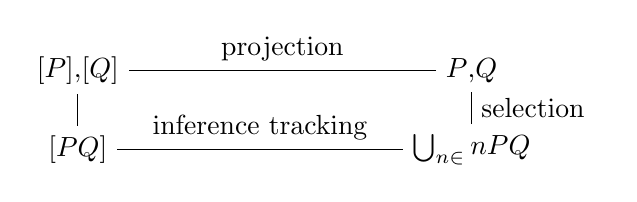
\begin{tikzpicture}
	\node   			(A)	{$\traces[P]$,$\traces[Q]$};
	\node[right of=A, xshift=40mm]	(B)	{$\trI{P}$,$\trI{Q}$};
	\node[below of=B]		(C)	{$\bigcup_{n\in\N}\tracesI{n}{P}{Q}$};
	\node[below of=A]		(D)	{$\traces[\procpar{P}{Q}]$};
	\path	(B)    edge node[anchor=south]  {projection}            (A)
		(C)    edge node[anchor=west, text width=15mm]   {selection}    (B)
		(D)    edge node[anchor=south]  {inference tracking}		(C);
	\path   (D)    edge[draw,decorate,decoration={snake, post=lineto, post length=4mm}] 
			    node[anchor=east]   {} (A);
\end{tikzpicture}
\caption{Visualization of the compositionality of the parallel operator (Part II).}
\label{fig_exp_comp_para2}
\end{figure}


With \refLem{lem_idx_trace_sets} we can show that there is a trace equality such that the traces of the parallel composition of processes without restriction and recursion is equal to the traces within the union of the inductive parallel composition sets.

\begin{lemma}[Compositionality of parallel composition]
\label{lem_compositionality_traces_para}
Given two processes $P,Q\in\procsresf\cap\procsrecf$. Then for the traces of a parallel composition
\[\traces[\procpar{P}{Q}]=\set[\exists\left(\cdot,s\right)\in\bigcup_{n\in\N}\tracesI{n}{P}{Q}]{s\in\tr}\]
holds.
\end{lemma}
\begin{prf}
Let $P,Q\in\procsresf\cap\procsrecf$. For the $\supseteq$-inclusion we know from \refLem{lem_idx_trace_sets} that for all $t\in\set[\exists\left(\cdot,s\right)\in\bigcup_{n\in\N\setminus\set{0}}\tracesI{n}{P}{Q}]{s\in\tr}$ there are $P_2,Q_2\in\procs$ such that $\ec{\procpar{P}{Q}}\bigstep{t}\ec{\procpar{P_2}{Q_2}}$ and so $t\in\traces[\procpar{P}{Q}]$ holds. Since with $t\in\set[\exists\left(\cdot,s\right)\in\tracesI{0}{P}{Q}]{s\in\tr}$ follows $t=\eseq$ and from \refLem{lem_empty_trace} we know that the empty trace is included in every trace set, we know that the fully inclusion holds.

%%%%%%%%%%%%%%%%%%%%%%%%%%%%%%%%%%%%%%%%%%%%%%%%%%%%% OTHER INCLUSION %%%%%%%%%%%%%%%%%%%%%%%%%%%%%%%%%%%%%%%%%%%%%%%%%%%%%%%%%%%%%%%%%%%%%%

For the $\subseteq$-inclusion, we induce over the length of a trace $s\in\traces[\procpar{P}{Q}]$:
\begin{description}
\item[Base case $s=\eseq$:] Since $\tracesI{0}{P}{Q} = \set[i_P,i_Q\in\N]{\left(\left(\left(i_P,0\right),\left(i_Q,0\right)\right),\eseq\right)}$, we know $s\in\set[\exists\left(\cdot,t\right)\in\bigcup_{n\in\N}\tracesI{n}{P}{Q}]{t\in\tr}$.

\item[Base case $s=\seq{\alpha}$ with $\alpha\in\actions\setminus\set{\tau}$:] From the definition of the big-step semantics (\refDef{def_bigstep_semantics}) we know that there are processes $P_1,P_2,Q_1,Q_2\in\procs$ such that $\ec{\procpar{P}{Q}}\bigstep{}\ec{\procpar{P_1}{Q_1}}\transs{\alpha}\ec{\procpar{P_2}{Q_2}}$. Since we have no restriction operator, we know the $\tau$ transitions within $\ec{\procpar{P}{Q}}\bigstep{}\ec{\procpar{P_1}{Q_1}}$ can either be produced from the \ecoml{} (respectively \ecomr{}) rule or from a $\tau$ prefix with the \eparl{} (respectively \eparr{}) rule. So there is a number $m\in\N$ and actions $\alpha_1,\ldots,\alpha_m\in\actions\setminus\set{\tau}$ and $\beta_1,\ldots,\beta_m\in\actions\setminus\set{\tau}$ such that $\ec{P}\bigstep{\seq{\alpha_1,\ldots,\alpha_m}}\ec{P_1}$ and $\ec{Q}\bigstep{\seq{\beta_1,\ldots,\beta_m}}\ec{Q_1}$ holds. Furthermore, there are just the \eparl{} and \eparr{} rule, which can produce the visible action $\alpha$. So we know $\ec{P_1}\transs{\alpha}\ec{P_2}$ or $\ec{Q_1}\transs{\alpha}\ec{Q_2}$ holds. Since both cases can be handled analogously, we just describe the first case. In this case we know $\ec{P}\bigstep{\seq{\alpha_1,\ldots,\alpha_m, \alpha}}\ec{P_2}$ and $Q_1=Q_2$ holds. Hence, there are numbers $i_P,i_Q\in\N$ with $\left(i_P,\seq{\alpha_1,\ldots,\alpha_m,\alpha}\right)\in\trI{P}$ and $\left(i_Q,\seq{\beta_1,\ldots,\beta_m}\right)\in\trI{Q}$. We also know that $\left(\left(\left(i_P,0\right),\left(i_Q,0\right)\right),\eseq\right)\in\tracesI{0}{P}{Q}$ holds so that we can step by step raise the counter for every $\alpha_i$ and $\beta_i$ with $i\in\set{1,\ldots,m}$ by taking in every step the COM conjunctive clause of \refDef{def_idx_trace_sets}. Hence, $\left(\left(\left(i_P,m\right),\left(i_Q,m\right)\right),\eseq\right)\in\tracesI{m}{P}{Q}$ holds. So we see that there is a tuple $\left(\left(\left(i_P,m+1\right),\left(i_Q,m\right)\right),\seq{\alpha}\right)\in\tracesI{m+1}{P}{Q}$, because the PL conjunctive clause of the definition of $\mathcal T_{m+1}$ is fulfilled. So we know $s\in\set[\exists\left(\cdot,t\right)\in\bigcup_{n\in\N}\tracesI{n}{P}{Q}]{t\in\tr}$ holds.

\item[Induction hypothesis:] For a given $n\in\N$, we know that for all $s\in\traces[\procpar{P}{Q}]$ with $\#(s)\leq{}n$ holds that $s\in\set[\exists\left(\cdot,t\right)\in\bigcup_{n\in\N}\tracesI{n}{P}{Q}]{t\in\tr}$.

\item[Induction step $n\mapsto n+1$:] So $\len{s}=n+1$. Again we know from the definition of the big-step semantics that there are processes $P_1,P_2,Q_1,Q_2\in\procs$ such that $\ec{\procpar{P}{Q}}\bigstep{s'}\ec{\procpar{P_1}{Q_1}}\transs{s_{n+1}}\ec{\procpar{P_2}{Q_2}}$ with $s'=\seq{s_1,\ldots,s_n}$ and $s_{n+1}\neq\tau$. Furthermore, since the cases of the empty trace and a trace with just one visible action are already done in the base cases, we consider $\len{s}\geq2$. Hence, we know $s'\neq\eseq$ holds. So there have to be processes $P_1',P_2',Q_1',Q_2'\in\procs$ with $\ec{\procpar{P}{Q}}\bigstep{\seq{s_1,\ldots,s_{n-1}}}\ec{\procpar{P_1'}{Q_1'}}\transs{s_n}\ec{\procpar{P_2'}{Q_2'}}\bigstep{}\ec{\procpar{P_1}{Q_1}}\transs{s_{n+1}}\ec{\procpar{P_2}{Q_2}}$. We now would like to find the suitable indices for $\left(\cdot,s'\right)\in\tracesI{x}{P}{Q}$ so that with this indices really the case $\ec{\procpar{P}{Q}}\bigstep{\seq{s_1,\ldots,s_{n-1}}}\ec{\procpar{P_1'}{Q_1'}}\transs{s_n}\ec{\procpar{P_2'}{Q_2'}}$ is described. So the visible action is the last step of the deduction and $P_2'$ and $Q_2'$ are really reached.

Since $\ec{\procpar{P}{Q}}\bigstep{s'}\ec{\procpar{P_1}{Q_1}}$ holds, we know with the induction hypothesis that $s'\in\set[\exists\left(\cdot,t\right)\in\bigcup_{n\in\N}\tracesI{n}{P}{Q}]{t\in\tr}$. Since $s'\neq\eseq{}$, we know there are $k_P,l_P,k_Q,l_Q,n'\in\N\setminus\set{0}$ such that $\left(\left(\left(k_P,l_P\right),\left(k_Q,l_Q\right)\right),s'\right)\in\tracesI{n'}{P}{Q}$. So, from \refLem{lem_idx_trace_sets}, we know there are tuple $\left(\left(\left(k_P,l_P'\right),\left(k_Q,l_Q'\right)\right),t'\right)\in\tracesI{n'-1}{P}{Q}$, $\left(k_P,r\right)\in\trI{P}$ and $\left(k_Q,t\right)\in\trI{Q}$ such that
\begin{align*}
	&\bigl(l_P=l_P'+1\wedge l_Q=b_Q'\wedge s'=\seqconc{t'}{\seq{r_{l_P}}}\wedge\exists R_1,R_2,S_1\in\procs: \\
 &\quad\ec{P}\bigstep{\seq{r_1,\ldots,r_{l_P}}}\ec{R_2}\wedge \ec{Q}\bigstep{\seq{t_1,\ldots,t_{l_Q}}}\ec{S_1}\wedge\ec{\procpar{P}{Q}}\bigstep{t'}\ec{\procpar{R_1}{S_1}}\transs{r_{l_P}}\ec{\procpar{R_2}{S_1}}\bigr) \\
	\vee&  \bigl(l_P=l_P'\wedge l_Q=l_Q'+1\wedge s'=\seqconc{t'}{\seq{t_{l_Q}}}\wedge\exists R_1,S_1,S_2\in\procs:\\
&\quad \ec{P}\bigstep{\seq{r_1,\ldots,r_{l_P}}}\ec{R_1}\wedge \ec{Q}\bigstep{\seq{t_1,\ldots,t_{l_Q}}}\ec{S_2}\wedge\ec{\procpar{P}{Q}}\bigstep{t'}\ec{\procpar{R_1}{S_1}}\transs{t_{l_Q}}\ec{\procpar{R_1}{S_2}} \bigr) \\
	\vee&  \bigl(l_P=l_P'+1\wedge l_Q=l_Q'+1\wedge r_{l_P}=\conj{t_{l_Q}}\wedge s'=t'\wedge\exists R_1,R_2,S_1,S_2\in\procs: \\
&\quad \ec{P}\bigstep{\seq{r_1,\ldots,r_{l_P}}}\ec{R_2}\wedge \ec{Q}\bigstep{\seq{t_1,\ldots,t_{l_Q}}}\ec{S_2}\wedge \ec{\procpar{P}{Q}}\bigstep{t'}\ec{\procpar{R_1}{S_1}}\tautrans\ec{\procpar{R_2}{S_2}}\bigr)
\end{align*}
holds. Hence, we know there are processes $R_2,S_2\in\procs$ with $\ec{\procpar{P}{Q}}\bigstep{s'}\ec{\procpar{R_2}{S_2}}$, but we do not know if these are the right indices such that $R_2=P_2'$, $S_2=Q_2'$ holds and $s_n$ is really the last deduction step. This is because arbitrary many $\tau$ steps could be performed after the visible action $s_n$ with the COM conjunctive clause of \refDef{def_idx_trace_sets} and nevertheless $s'\in\set[\exists\left(\cdot,t\right)\in\bigcup_{n\in\N}\tracesI{n}{P}{Q}]{t\in\tr}$ would hold. But we can revert every of the excessive $\tau$ steps, so we know there exists $m,j_P',j_P'',j_Q',j_Q''\in\N$ with $m\leq{}n'$,$j_P''\leq{}l_P'$ and $j_Q''\leq{}l_Q'$ such that $\left(\left(\left(k_P,j_P'\right),\left(k_Q,j_Q'\right)\right),s'\right)\in\tracesI{m}{P}{Q}$, $\left(\left(\left(k_P,j_P''\right),\left(k_Q,j_Q''\right)\right),t'\right)\in\tracesI{m-1}{P}{Q}$, $\left(k_P,r\right)\in\trI{P}$ and $\left(k_Q,t\right)\in\trI{Q}$ exists such that
\begin{align*}
	&\bigl(j_P'=j_P''+1\wedge j_Q'=j_Q''\wedge r_{j_P'}=s_n \wedge s'=\seqconc{t'}{\seq{s_n}} \\
&\quad\wedge\ec{P}\bigstep{\seq{r_1,\ldots,r_{j_P'}}}\ec{P_2'}\wedge \ec{Q}\bigstep{\seq{t_1,\ldots,t_{j_Q'}}}\ec{Q_1'}\wedge\ec{\procpar{P}{Q}}\bigstep{t'}\ec{\procpar{P_1'}{Q_1'}}\transs{s_n}\ec{\procpar{P_2'}{Q_1'}}\bigr)\\
\vee&  \bigl(j_P'=j_P''\wedge j_Q'=j_Q''+1\wedge t_{j_Q'}=s_n \wedge s'=\seqconc{t'}{\seq{s_n}} \\
&\quad \wedge \ec{P}\bigstep{\seq{r_1,\ldots,r_{j_P'}}}\ec{P_1'}\wedge \ec{Q}\bigstep{\seq{t_1,\ldots,t_{j_Q'}}}\ec{Q_2'}\wedge\ec{\procpar{P}{Q}}\bigstep{t'}\ec{\procpar{P_1'}{Q_1'}}\transs{s_n}\ec{\procpar{P_1'}{Q_2'}} \bigr)
\end{align*}
holds. The conjunctive clause which handles the communication case is not satisfiable since the last step has to be a visible action and is due to that omitted.

Since $t'=\seq{s_1,\ldots,s_{n-1}}$, we found the suitable indices such that 
\[\ec{\procpar{P}{Q}}\bigstep{\seq{s_1,\ldots,s_{n-1}}}\ec{\procpar{P_1'}{Q_1'}}\transs{s_n}\ec{\procpar{P_2'}{Q_2'}}\]
holds. We now have to raise the indices for the $\tau$ steps within $\ec{\procpar{P_2'}{Q_2'}}\bigstep{}\ec{\procpar{P_1}{Q_1}}$ and the visible action $\ec{\procpar{P_1}{Q_1}}\transs{s_{n+1}}\ec{\procpar{P_2}{Q_2}}$. Again we know that the visible action $s_{n+1}$ must be produced from the \eparl{} (respectively \eparr{}) rule and since both cases are similar, we concentrate on the \eparl{} case.

To find the suitable indices such that $\ec{\procpar{P}{Q}}\bigstep{s'}\ec{\procpar{P_2'}{Q_2'}}\bigstep{}\ec{\procpar{P_1}{Q_1}}\transs{s_{n+1}}\ec{\procpar{P_2}{Q_2}}$ holds, we can -- as in the second base case -- raise the indices for every $\tau$ step within $\ec{\procpar{P_2'}{Q_2'}}\bigstep{}\ec{\procpar{P_1}{Q_1}}$ with the COM conjunctive clause. But in this case, we do not know, how $r$ and $t$ look like. If they are long enough so that every action which is needed in the premise of the \ecoml{} (respectively \ecomr{}) rule to deduct the $\tau$ steps within $\ec{\procpar{P_2'}{Q_2'}}\bigstep{}\ec{\procpar{P_1}{Q_1}}$ and as well the action $s_{n+1}$ is contained, then we can just raise the counter. Otherwise, if $r$ and $t$ do not contain every needed action, we know $\ec{\procpar{P}{Q}}\bigstep{\seq{s_1,\ldots,s_{n-1}}}\ec{\procpar{P_1'}{Q_1'}}\transs{s_n}\ec{\procpar{P_2'}{Q_2'}}\bigstep{}\ec{\procpar{P_1}{Q_1}}\transs{s_{n+1}}\ec{\procpar{P_2}{Q_2}}$ holds and that those steps can just be performed by applying the \eparl{} (respectively \eparr{}) or \ecoml{} (respectively \ecomr) rules. Hence, we know, there have to be traces $u,v\in\tr$ with $\ec{P}\bigstep{r}\ec{P_2'}\bigstep{\seqconc{u}{\seq{s_{n+1}}}}\ec{P_2}$ and $\ec{Q}\bigstep{t}\ec{Q_2'}\bigstep{v}\ec{Q_2}$, since we consider the \eparl{} case. Hence, we know that nothing changes, if we use the tuple $\left(i_P,u'\right)\in\trI{P}$ with $u'\define\seqconc{\seqconc{r}{u}}{s_{n+1}}$ instead of $\left(k_P,r\right)\in\trI{P}$ and $\left(i_Q,v'\right)\in\trI{Q}$ with $v'\define\seqconc{t}{v}$ instead of $\left(k_Q,t\right)\in\trI{Q}$. With this we can, as in the base case, increase $j_P'$ and $j_Q'$ by one for every $\tau$ deduction within $\ec{\procpar{P_2'}{Q_2'}}\bigstep{}\ec{\procpar{P_1}{Q_1}}$. So we found the suitable numbers $m',i_P,j_P,i_Q,j_Q\in\N$ such that $\left(\left(\left(i_P,j_P\right),\left(i_Q,j_Q\right)\right),s'\right)\in\tracesI{m'}{P}{Q}$, $\left(i_P,u'\right)\in\trI{P}$ and $\left(i_Q,v'\right)\in\trI{Q}$, with $m'\geq{}m$, $j_P\geq{}j_P'$ and $j_Q\geq{}j_Q'$ holds for $\ec{\procpar{P}{Q}}\bigstep{\seq{s_1,\ldots,s_{n-1}}}\ec{\procpar{P_1'}{Q_1'}}\transs{s_n}\ec{\procpar{P_2'}{Q_2'}}\bigstep{}\ec{\procpar{P_1}{Q_1}}$. Hence, we know that $\left(\left(\left(i_P,j_P+1\right),\left(i_Q,j_Q\right)\right),s\right)\in\tracesI{m'+1}{P}{Q}$ holds, since the PL conjunctive clause holds, because of considering the \eparl{} case. So $s\in\set[\exists\left(\cdot,t\right)\in\bigcup_{n\in\N}\tracesI{n}{P}{Q}]{t\in\tr}$ holds.
\end{description}
So we proved that the parallel composition is compositional for processes without restriction and recursion.
\end{prf}

The next section dealts with the last unconsidered operator of recursion-free \picalc{} processes.
